% This must be in the first 5 lines to tell arXiv to use pdfLaTeX, which is strongly recommended.
\pdfoutput=1
% In particular, the hyperref package requires pdfLaTeX in order to break URLs across lines.

\documentclass[12pt]{article}

% Remove the "review" option to generate the final version.
\usepackage[review]{ACL2023}

% Standard package includes
\usepackage{times}
\usepackage{latexsym}

% For proper rendering and hyphenation of words containing Latin characters (including in bib files)
\usepackage[T1]{fontenc}
% For Vietnamese characters
% \usepackage[T5]{fontenc}
% See https://www.latex-project.org/help/documentation/encguide.pdf for other character sets

% This assumes your files are encoded as UTF8
\usepackage[utf8]{inputenc}

% This is not strictly necessary, and may be commented out.
% However, it will improve the layout of the manuscript,
% and will typically save some space.
\usepackage{microtype}

% This is also not strictly necessary, and may be commented out.
% However, it will improve the aesthetics of text in
% the typewriter font.
\usepackage{inconsolata}
\usepackage{graphicx}
\usepackage{float}
\usepackage{booktabs} % For better table formatting
\usepackage{multirow}
\usepackage{array}

% If the title and author information does not fit in the area allocated, uncomment the following
%
%\setlength\titlebox{<dim>}
%
% and set <dim> to something 5cm or larger.

\title{Harnessing Ensemble Learning to Shape Consumer Choices: A Yelp Sentiment Analysis Approach}

\author{Nomita Chandra \and Kevin Kuc \and Weijie Yang \\
        nchandra4@berkeley.edu \\ kkuc100@berkeley.edu \\ raphael.yang@berkeley.edu}

\begin{document}
\maketitle
\begin{abstract}
  In the current digital landscape, online presence and customer reviews play a crucial role in shaping consumer perceptions and influencing purchasing decisions. Platforms such as Yelp have become essential, offering a comprehensive medium for consumers to discover, connect with, and transact with local businesses. This increased reliance on Yelp reviews has significantly impacted business reputations and success. Consequently, the growing volume of reviews necessitates the development of efficient and accurate methods for their analysis. In this paper, we proposed to perform sentiment classification on Yelp reviews using the \href{https://huggingface.co/datasets/Yelp/yelp_review_full}{Yelp Review Dataset} from Hugging Face, originally constructed by Xiang Zhang from the Yelp Dataset Challenge 2015. We utilized the Yelp Review Dataset, comprising 650,000 training and 50,000 test reviews labeled from 1 to 5 stars. Sentiment analysis of customer reviews was crucial for businesses to gauge customer satisfaction, identify improvement areas, enhance customer experiences, address negative feedback promptly, and reinforce positive service aspects. We employed RoBERTa, Bert-large-uncased, and Flan-T5 as base models, leveraging Ensemble Learning to enhance model performance. RoBERTa’s Masked Language Modeling (MLM) enabled comprehensive information extraction, Bert-large-uncased’s bi-directional training approach considered both left and right contextual information, and Flan-T5’s encoder extracted semantic meanings to facilitate inference. Ensemble Learning integrated the outputs of these models, as illustrated in the algorithmic architecture. [Details on the methods used for testing will be outlined here.] [Results of the sentiment classification testing will be presented here.]
\end{abstract}


\section{Introduction}
In today’s digital era, a business's online presence and customer reviews play a crucial role in shaping consumer perceptions and driving purchasing decisions \citep{luca2016reviews}. Yelp, a prominent platform for discovering, connecting with, and transacting with local businesses, serves as a key resource for consumers seeking accurate information to guide their choices \citep{lee2014impact}. With its significant impact on consumer behavior, businesses worldwide strive to achieve higher ratings and positive feedback. As the volume of reviews continues to grow, the demand for efficient and precise methods to analyze and classify this textual data has never been greater \citep{pang2008sentiment}.

\subsection{Introduction to NLP}
Natural Language Processing (NLP) has emerged as a powerful tool for automating text analysis, enabling businesses to extract meaningful insights from vast amounts of data \citep{jurafsky2020speech}. NLP, a subfield of Artificial Intelligence, involves breaking down or tokenizing text, embedding it, and using these embeddings as inputs for downstream models \citep{manning1999foundations}. This technology allows for sophisticated analysis of textual data, facilitating a deeper understanding of consumer sentiments.

\subsection{Importance}
Our project, "Harnessing Ensemble Learning to Shape Consumer Choices: A Yelp Sentiment Analysis Approach" focuses on classifying the sentiment of Yelp reviews. Utilizing the Yelp Review Dataset from Hugging Face, originally curated by Xiang Zhang during the Yelp Dataset Challenge 2015 \citep{zhang2015sensitivity}, our model is designed to infer sentiment ratings for Yelp reviews. Understanding customer sentiment is vital for businesses, as it provides insights into customer satisfaction, highlights areas for improvement, and helps address feedback effectively. By leveraging sentiment analysis, businesses can enhance customer experiences, promptly address negative comments, and reinforce positive aspects of their services \citep{pang2008sentiment}.

\section{Background}

\subsection{Challenges}
One of the primary challenges in our project is preprocessing the data to ensure its relevance and usability for sentiment analysis. The dataset consists of reviews of varying lengths, necessitating the truncation and padding of reviews to create uniform input sizes while preserving their sentiment. Additionally, we need to consider implementing data augmentation techniques to expand our dataset, enabling our model to train on a larger and more diverse set of data. Lastly, a significant challenge is developing the machine learning model's capability to extract semantic meaning from lengthy reviews.

\subsection{Dataset}
We utilized the \href{https://huggingface.co/datasets/Yelp/yelp_review_full}{Yelp Review Dataset} available on Hugging Face, which is constructed by randomly taking 130,000 training samples and 10,000 testing samples for each review star from 1 to 5. In total there are 650,000 trainig samples and 50,000 testing samples. For our analysis, we considered three distinct data configurations:

\begin{itemize}
  \item \textbf{Original Five-Class Classification:} We analyzed the dataset with its original five-star rating scale. This approach is anticipated to have the lowest accuracy due to the inherent difficulty in distinguishing between closely related classes, such as between 1 and 2 stars, as well as between 4 and 5 stars.

  \item \textbf{Three-Class Classification:} We reclassified the reviews into three categories: 'negative' for 1-2 stars, 'positive' for 4-5 stars, and 'mixed' for 3 stars. Reviews with 1-2 stars were grouped together as they predominantly contain negative critiques, while 4-5 stars generally reflect positive feedback. Reviews with a 3-star rating represent a mix of both positive and negative observations. This approach is expected to yield intermediate accuracy, as it simplifies the classification task compared to the original five-class problem.

  \item \textbf{Binary Classification:} We reclassified the reviews into two categories: 'negative' for 1-2 stars and 'positive' for 4-5 stars, excluding 3-star reviews from the dataset. This binary classification is hypothesized to provide the highest accuracy, as it removes the ambiguity associated with the 'mixed' category.
\end{itemize}

\section{Methodology}
This section describes our approach, including data processing, complete model architecture as well as output summarization technique for applications.

% Methodology image inclusion
\begin{figure}[H]
  \centering
  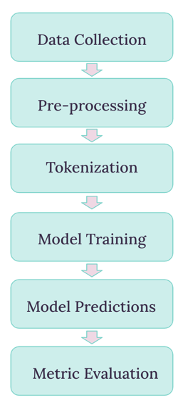
\includegraphics[width=0.2\textwidth, height=0.3\textheight]{./methodology.jpg}
  \caption{Comprehensive overview of our approach, detailing each stage from Data Collection through Metric Evaluation.}
  \label{fig:example}
\end{figure}

\section{Methods}

\subsection{Data Processing}
To prepare the Yelp Review Dataset for analysis, several preprocessing steps were conducted to ensure data quality and balance. Initially, the dataset, sourced from Hugging Face, was subjected to word count computation for each review. Reviews with word counts fewer than 100 or more than 200 were excluded. This range was chosen to filter out reviews that were too short, which often signify low-quality content, and overly lengthy reviews, which can introduce noise and complexity without providing additional value (Pang and Lee, 2004; Liu, 2012). Following this, to create a balanced training and test set, random sampling was applied to select an equal number of samples from each label. These preprocessing steps were critical and necessary in ensuring that the dataset was of high quality, balanced, and representative of various sentiment categories, thus facilitating more accurate and reliable analysis and model training.

\subsection{Baseline Model}
To establish a foundational approach for classifying Yelp reviews, we implemented a bag-of-words (BoW) model in conjunction with a Naive Bayes classifier. This approach was chosen for its balance of simplicity and effectiveness in initial evaluations \citep{rish2001empirical}. The Naive Bayes classifier, grounded in Bayes' Theorem, is renowned for its computational efficiency and rapid processing capabilities. The model operates by tokenizing the text into individual words, which are then represented as discrete features. Each word token contributes to the calculation of the posterior probability of a given sentiment class based on its frequency and the class's prior probability. The Naive Bayes algorithm combines these token-based probabilities to infer the sentiment of the entire review. Given that reviewers often infuse their text with a high degree of passion and emotion, we anticipated that this approach would yield accurate results, as the BoW model is well-suited to capture these sentiments through the frequency and presence of emotionally charged words.

\subsection{Baseline Results}
Our results demonstrated the model’s performance across different classification schemes. For the original five-class classification, the BoW model achieved an accuracy of 0.52, with stars 1 and 2 exhibiting the lowest F1-scores of 0.44 and 0.47, respectively. In the three-class classification, the model achieved an accuracy of 0.68, though the neutral class had the lowest F1-score of 0.61. The binary classification model performed notably better, with an accuracy of 0.88, and both categories showed equal accuracy. The assumption of feature independence allows for straightforward computation, but to further refine our model's performance, the next phase involved incorporating additional contextual information and exploring more sophisticated methods \citep{rish2001empirical}.

\subsection{Upstream Base Model Selection}
For the classification tasks, we employed RoBERTa (Robustly optimized BERT approach) and DeBERTa (Decoding-enhanced BERT with disentangled attention) as our upstream base models for the whole model architecture. We take the hidden layers from both two BERT models and connected with dense layers as well as a softmax layer for our downstream classification task. 

\subsection{RoBERTa}
RoBERTa is an enhanced version of BERT that has been optimized through longer training with larger batches, removal of the next sentence prediction objective, and training on a larger dataset \citep{liu2012sentiment}. These improvements enable RoBERTa to achieve superior performance by better capturing the nuances of language, making it particularly suitable for sentiment analysis and text classification tasks where understanding context and sentiment from text is crucial \citep{liu2012sentiment}. We expect that Its great capabilities in sentiment comprehension can identify people’s preferences and attitudes entailed in the reviews and generate predictions with qualities.

\subsection{DeBERTa}
DeBERTa introduces disentangled attention mechanisms and an enhanced mask decoder, which allow it to more effectively encode semantic information and improve the model's performance on downstream tasks \citep{he2020deberta}. The disentangled attention mechanism separates the content and position information, leading to a more refined understanding of the text, which is beneficial for accurately classifying reviews that may have subtle sentiment cues \citep{he2020deberta}. Subtle sentiment detection ability is crucial to our task as we classify the review in a star-rating model. It is easy to identiy “star 0” and “star 4”. However, the boundary and difference between “star 0” and “star 1” is ambiguous as they both show negative sentiment signals in reviews. How to define the degree of negative sentiment requires high sensitivity to subtle sentiment change for the model.

By leveraging the strengths of RoBERTa and DeBERTa, we aimed to enhance the predictive performance and reliability of our classification models, ensuring they could handle the complexities of the Yelp Review Dataset effectively. Besides, we employed the Text-to-Text Transfer Transformer (T5) model for summarizing our modeling results. The T5 model transforms all NLP tasks into a text-to-text format, including summarization. Its strength lies in its extensive pre-training, allowing it to generate coherent and concise summaries. From the perspective of users who care about the reviews and hope to gain insights from the reviews to improve the products as well as mitigate existing issues, our who model architecture and solution needs to generate summarized outputs to highlight the key useful information to the users instead of passing them long reviews.

\subsection{Ensemble}
Ensemble learning is an effective approach to mitigate overfitting by averaging biases and variances from multiple models, thus enhancing overall model performance (Opitz and Maclin, 1999). It also corrects the errors made by individual weak learners, leading to better predictive accuracy \citep{schapire1990strength}. Figure X displays our whole model architecture. First, we preprocessed the dataset and tokenized the dataset with DeBERTa and RoBERTa’s tokenizers correspondingly. Then, we customized both BERT models by taking their hidden states and importing to dense layers and softmax layers to get the predictions. To better integrate and boost the prediction capbilities, as well as taking the strength of both BERT models, we employed multiple Ensemble Learning approaches including averaging, stacking, voting, MLP, random forest, decision tree, and gradient boosting. Specifically, we take the softmax layers with the size of [5*batch size] from both two models and compute the average value of the two vectors as the input for ensemble learning classifier to get the final prediction. Above models are fine-tuned to get the best performance version. Then, T5 is adopted here to take the outputs for each class and summarize the long reviews into short sentences and keywords.

% Model_architecture image inclusion
\begin{figure*}[h!]
  \centering
  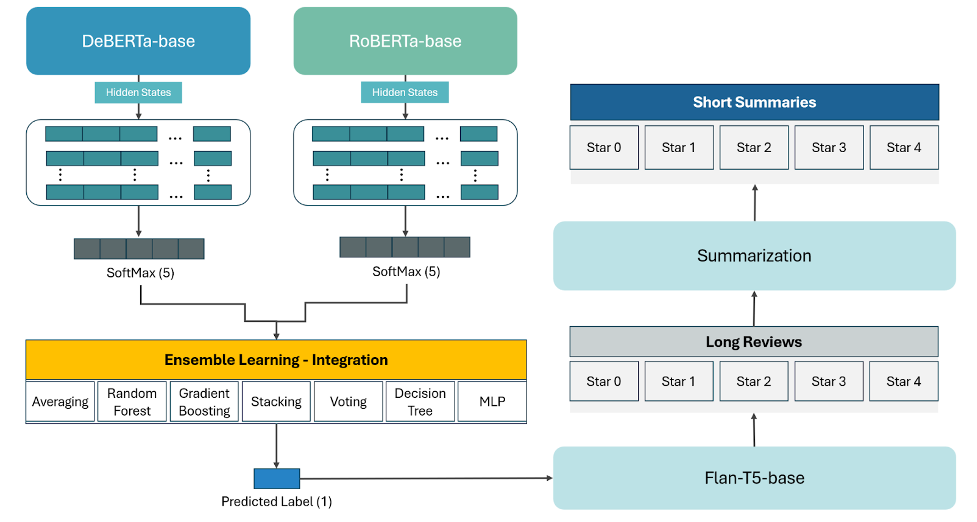
\includegraphics[width=1.0\textwidth, height=0.3\textheight]{./model_architecture.png}
  \caption{Whole model architecture by using ensemble learning to consolidate the model predictions from both DeBERTa and RoBERTa.}
  \label{fig:model_architecture}
\end{figure*}

\begin{table*}[h!]
  \centering
  \small % Reduces the font size
  \begin{tabular}{|p{3cm}|p{4.5cm}|>{\centering\arraybackslash}p{1.5cm}|>{\centering\arraybackslash}p{1.5cm}|>{\centering\arraybackslash}p{1.5cm}|>{\centering\arraybackslash}p{1.5cm}|}
    \hline
    \textbf{Model} & \textbf{Best Training Hyperparameters} & \textbf{Test set Macro F1} & \textbf{Test set Micro F1} & \textbf{Test set Precision} & \textbf{Test set Recall} \\
    \hline
    Naive Bayes (Baseline) & - & - & - & - & - \\
    \hline
    RoBERTa-base (Customized) & \begin{tabular}[c]{@{}l@{}}Learning rate = 1e-5, \\ Hidden layers size = 100, \\ Dropout = 0.20, \\ Max length = 200, \\ Epoch = 4\end{tabular} & 0.58 & 0.58 & 0.59 & 0.58 \\
    \hline
    DeBERTa-base (Customized) & \begin{tabular}[c]{@{}l@{}}Learning rate = 1e-5, \\ Hidden layers = 200, \\ Dropout = 0.20, \\ Max length = 200, \\ Epoch = 3\end{tabular} & 0.58 & 0.58 & 0.62 & 0.58 \\
    \hline
    Ensemble Learning (Averaging) & - & 0.59 & 0.59 & 0.61 & 0.59 \\
    \hline
    Ensemble Learning (Random Forest) & Max depth = 2 & 0.62 & 0.62 & 0.63 & 0.62 \\
    \hline
    Ensemble Learning (Decision Tree) & Max depth = 3 & 0.61 & 0.61 & 0.62 & 0.61 \\
    \hline
    Ensemble Learning (MLP) & \begin{tabular}[c]{@{}l@{}}Max iteration = 500, \\ Learning rate = 0.005\end{tabular} & 0.62 & 0.62 & 0.62 & 0.62 \\
    \hline
    Ensemble Learning (Gradient Boosting) & \begin{tabular}[c]{@{}l@{}}Estimator = 200, \\ Learning rate = 0.005\end{tabular} & 0.58 & 0.58 & 0.59 & 0.58 \\
    \hline
    Ensemble Learning (Stacking) & \begin{tabular}[c]{@{}l@{}}Random Forest (estimator = 10), \\ MLP (max iteration = 500, \\ learning rate = 0.005), \\ Gradient Boosting (estimator = 200, \\ learning rate = 0.005)\end{tabular} & 0.55 & 0.55 & 0.57 & 0.55 \\
    \hline
    Ensemble Learning (Voting) & \begin{tabular}[c]{@{}l@{}}Random Forest (estimator = 10), \\ MLP (max iteration = 500, \\ learning rate = 0.005), \\ Gradient Boosting (estimator = 200, \\ learning rate = 0.005)\end{tabular} & 0.61 & 0.60 & 0.61 & 0.60 \\
    \hline
  \end{tabular}
  \caption{Grid search result for baseline model, BERT models, and ensemble learning.}
  \label{tab:model_performance}
\end{table*}

\section{Results and Discussion}
We conducted grid search by experimenting with different hyperparameter sets to find the best performance model for Naive Bayes (baseline), RoBERTa-base as well as DeBERTa-base. After finding best BERT models, we also experimented with different ensemble learning approaches including averaging, stacking, voting, random forest, decision tree as well multi-linear perceptrons to seek the top ensemble learning performers. Table X displays our grid search result.

\section{Conclusion}

\section*{Limitations}
Our study encountered several limitations that could affect the relevance and generalizability of our model. One notable constraint was our decision to use a dataset from 2015 instead of the Yelp API. While this choice was made to manage dataset availability, it inherently limits the temporal relevance of our model. Language and user sentiment evolve over time, and the static nature of our dataset may prevent the model from capturing contemporary language use and emerging trends in user reviews.

Another limitation is our focus solely on English reviews. By concentrating on a single language, the model’s applicability to multilingual contexts is restricted. This singular linguistic focus may reduce the model's generalizability and effectiveness in diverse, multilingual environments. Future research could benefit from including a range of languages to enhance the model's robustness and broader applicability.

Additionally, we imposed a constraint on text length to ensure dataset consistency and manageability. Specifically, we limited reviews to within 300 characters above or below the average text length. This filtering approach resulted in the exclusion of reviews significantly longer or shorter than this range. While this was intended to maintain a uniform dataset, it may have inadvertently omitted valuable information from reviews outside this length range. This exclusion could impact the model’s ability to handle diverse review lengths and capture potentially significant nuances.

Addressing these limitations in future work could improve the relevance, inclusivity, and accuracy of sentiment analysis models for Yelp reviews and similar applications.

\section*{Ethics Statement}

In alignment with the ACL Ethics Policy \citep{acl2023ethics}, we present the following ethics statement for our Yelp Sentiment Analysis project. Our research focuses on analyzing sentiment in Yelp reviews, a task that inherently involves understanding and interpreting user-generated content. We recognize the following ethical considerations and steps taken:

\begin{itemize}
    \item \textbf{Data Privacy and Confidentiality}: We use publicly available Yelp reviews, ensuring that our analysis respects user privacy. All personal identifiers are anonymized, and we adhere to best practices in data handling to prevent misuse of sensitive information.

    \item \textbf{Bias and Fairness}: Sentiment analysis models are prone to biases that can affect the accuracy of predictions. We are committed to addressing and mitigating biases in our models. We continuously evaluate our model's performance across diverse demographic groups and make adjustments to minimize any disparate impact.
    
    \item \textbf{Transparency and Reproducibility}: We strive for transparency in our methodology and results. All code and data (within permissible limits) used in our research will be made available to the community to ensure reproducibility and to facilitate further research.
    
    \item \textbf{Ethical Use of Technology}: Our work is intended to contribute positively to the understanding of user sentiment in public reviews. We do not support or condone the misuse of sentiment analysis technology for manipulative or deceptive purposes.
    
    \item \textbf{Impact and Implications}: We acknowledge that sentiment analysis can influence public perception and decision-making. We are committed to ensuring that our research does not propagate misinformation or contribute to unfair practices. We encourage stakeholders to use our findings responsibly and ethically.
\end{itemize}

By addressing these considerations, we aim to uphold the highest standards of ethical practice in our research and contribute positively to the field.

\section*{Acknowledgements}
I would like to extend my sincere gratitude to the following individuals for their invaluable contributions:
\begin{itemize}
  \item Peter Grabowski
  \item Natalie Ahn
  \item Amit Bhattacharyya
  \item Jennifer Zhu
  \item Mike Tamir
  \item Paul Spiegelhalter
  \item Mark Butler
\end{itemize}
Their support and insights have significantly enhanced this research. Thank you all for your time and assistance.

\bibliography{anthology,custom}
\bibliographystyle{acl_natbib}

\nocite{liu2019roberta, devlin2019bert, chung2022scaling, huggingface_yelp, opitz1999popular, schapire1990strength, he2020deberta, hu2004mining, liu2012sentiment, pang2004sentimental, pang2002thumbs, rish2001empirical,acl2023ethics}

\appendix

\section{Example Appendix}
\label{sec:appendix}

This is a section in the appendix.

\end{document}
